\section{Implémentation, tests et résultats}
\subsection{Structuration}
Le code du \texttt{SeedDB} est composé de quatre classes qui implémentent en python les algorithmes présentés dans le chapitre précédent.

La classe \texttt{SeedDB} est composée de fonctions telles:
%Le code est composé de fonctions (nouvelle version avec les threads, héritage):
\begin{enumerate}
\item \texttt{\_\_init\_\_}
\item \texttt{request\_snmp\_parameters}
\item \texttt{check\_snmp}
\item \texttt{device\_discovery}
%\item \texttt{get\_indirect\_next\_hop}
%\item \texttt{device\_grouping}
%\item \texttt{get\_local\_net\_address}
\item \texttt{get\_device\_type}
\item \texttt{create\_bulk\_format}
\item \texttt{catch\_exit}
\end{enumerate}
Cette classe \texttt{SeedDB} dépend de trois classes qui lui offrent des fonctionnalités spécifiques:
\begin{enumerate}
\item \texttt{DeviceGrouping} pour le filtrage des synonymes dans le réseau.
\item \texttt{GetIndirectNextHop} pour lé découverte de tous les routeurs du réseau.
\item \texttt{GetLocalNetAddress} pour la découverte des équipements actif dans un réseau local.
\end{enumerate}
Aussi les modules suivantes sont importés:
\begin{itemize}
\item \texttt{nav.Snmp}: utilisation du module \emph{SNMP} du NAV.
\item \texttt{buildconf}: utilisation du module \texttt{buildconf} de NAV pour retrouver automatiquement le répertoire des fichiers de logs. 
\item \texttt{signal}: interception action de l'utilisateur comme l'arrêt prématuré du script avec la commande \texttt{Control-C}.
%\item \texttt{sys}: code de sortie du programme.
\item \texttt{datetime}: personnalisation du nom du fichier de bulk crée à la seconde près.
\item \texttt{os}: utilisation des ressources du système, comme la création d'un répertoire pour la sauvegarde des fichiers de bulk.
\item \texttt{IPy}: vérification de la validité IPv4 et IPv6 de l'adresse donnée pour le \texttt{seedRouter}.
\item \texttt{logging}: création de logs suivant le modèle de Python.
\item \texttt{threading}: utilisation du module \emph{threading} de la classe \emph{thread}.
\end{itemize}

Des variables de portée globale sont créés pour contenir les \texttt{OID}s des \emph{MIBs} nécessaires pour la découverte des types hôtes dans le réseau.
\begin{itemize}
\item \texttt{sys\_service="1.3.6.1.2.1.1.7"} pour identifier les types d'équipements dans le réseau par la classe mère \texttt{SeedDb}.
\item \texttt{ip\_route\_next\_hop="1.3.6.1.2.1.4.21.1.7"} pour récupérer tous les autres routeurs auxquels est connecté un équipement (classe \texttt{GetIndirectNextHop}).
\item \texttt{ip\_route\_type="1.3.6.1.2.1.4.21.1.8"} pour ne récupérer que les \emph{NextHop} de type \emph{indirect} (classe \texttt{GetIndirectNextHop}).
\item \texttt{ip\_forwarding="1.3.6.1.2.1.4.1"} pour filtrer les PC routeurs des simples PC (classe \texttt{SeedDb}).
\item \texttt{ip\_ad\_ent\_addr="1.3.6.1.2.1.4.20.1.1"} pour récupérer tous les adresses IP de tous les interfaces d'un équipement (classe \texttt{DeviceGrouping}).
\item \texttt{ip\_net\_to\_media\_net\_address="1.3.6.1.2.1.4.22.1.3"} pour récupérer les adresses IP des équipements appartenant au même réseau local (classe \texttt{GetLocalNetAddress}).
\item \texttt{dot1d\_bridge="1.3.6.1.2.1.17"} pour identifier les switchs (classe \texttt{SeedDb}).
\end{itemize}
Aussi les variables globales \texttt{my\_room} et \texttt{my\_org} initialisées avec respectivement les valeurs \emph{myroom} et \emph{myorg}.

%Le code est disponible à l'annexe \nameref{codeSource}.

\subsection{La classe SeebDB}
C'est la classe principale qui importe tous les modules nécessaires et appel ses méthodes et autres classes en fonction du déroulement du processus. Comme méthodes de cette classe nous avons:
\subsubsection{\_\_init\_\_}
La méthode \texttt{\_\_init\_\_} est le constructeur de la classe \texttt{SeedBD}. \'A l'appel de la classe, le constructeur demande deux informations à l'utilisateur: l'adresse IP du \emph{Starting point} et la version de SNMP à utiliser. Si une de ses informations est incorrectes, le script s'arrête. De même, si les paramètres de sécurité ne sont pas correctes pour le \emph{Starting point}, le script s'arrête.

En fonction de la version valide de SNMP choisie, la méthode \texttt{request\_snmp\_parameters} est appelée.
 
\subsubsection{request\_snmp\_parameters}
La fonction \texttt{request\_snmp\_parameters} récupère les informations de sécurité en fonction de la version de SNMP choisi précédemment. Pour les versions 1 et 2, seule le \texttt{community} est nécessaire. Pour la version 3, sont nécessaires les informations suivantes: 
\begin{itemize}
\item \texttt{username}: identifiant d'authentification,
\item \texttt{security level}: niveau de sécurité entre \emph{noAuthnoPriv,authnoPriv et authPriv},
\item \texttt{authentifiaction protocol}: protocole d'authentification entre \emph{MD5 et SHA},
\item \texttt{password}: mot de passe d'authentification,
\item \texttt{privacy protocol}: protocole de cryptage, entre \emph{DES et AES},
\item \texttt{passphrase}: clé de cryptage.
\end{itemize}

Vu que NAV ne supporte pas encore la version 3 de SNMP, nous n'implémenterons que les versions 1 et 2 du protocole.

En fonction de la version choisie (1 ou 2), la méthode \texttt{check\_snmp} intervient.

\subsubsection{check\_snmp}
L'objectif de la méthode \texttt{check\_snmp} est de s'assurer que les paramètres de sécurités fournis sont bien valide pour le \emph{seedRouter} donné. Dans le cas des versions 1 et 2, seul le \texttt{community} est vérifié. La vérification passe par l'envoie d'une requête SNMP sur le \emph{MIB} \texttt{sysDescr} (OID: \texttt{1.3.6.1.2.1.1.1}). Cet OID est utilisé de manière native par NAV pour s'assurer de la validité des paramètres de sécurités SNMP au niveau des équipements. Dans une dynamique de compatibilité avec le NAV, nous utilisons également cet OID comme critère d'évaluation.

Si l'équipement répond à la requête SNMP \texttt{getRequest}, alors la fonction  \texttt{device\_discovery} prend le relais.

\subsubsection{device\_discovery}
C'est la fonction principale (la plus importante) de notre implémentation. Elle inclue les classes \texttt{GetIndirectNextHop}, \texttt{DeviceGrouping}, \texttt{GetLocalNetAddress} et les méthodes \texttt{get\_device\_type} et \texttt{create\_bulk\_format}. La méthode \texttt{device\_discovery} permet d'avoir dans un fichier \emph{txt}, la liste des équipements du réseau au format de NAV.

Pour gérer les successions d'accès à la ressource commune qu'est le tableau des équipements du réseau, un sémaphore est mis en place à travers la variable \texttt{lock = threading.Lock()}

Grâce aux résultats qui lui sont fournis par les classes \texttt{GetIndirectNextHop}, \texttt{DeviceGrouping}, \texttt{GetLocalNetAddress}, la méthode \texttt{device\_discovery} dispose dans un tableau la liste complète de tous les équipements uniques dans le réseau. Cet tableau est alors utilisé par les méthodes \texttt{get\_device\_type} et \texttt{create\_bulk\_format}.

\subsubsection{get\_device\_type\\}
L'identification des hôtes est assurée par la méthode \texttt{get\_device\_type} en utilisant les \emph{MIB}s \texttt{sysService}, \texttt{ipForwarding} et \texttt{dot1dBridge}. En fonction des résultats obtenus par \texttt{getRequest} pour chaque \emph{MIB}, un type d'équipement conforme aux types d'équipements\footnote{\url{http://nav.uninett.no/categoriesandtypes}} du NAV est détecté.
\subsubsection{create\_bulk\_format\\}
Cette dernière méthode du \texttt{device\_discovery} permet de générer un fichier texte contenant les informations conforme au  \emph{Level 1: Minimum requirements}\footnote{\url{http://nav.uninett.no/seedessentials}} dans le répertoire \texttt{/tmp/nav}. Le fichier est identifié à la seconde près par son nom composé en partie par l'année, le mois, le jour, l'heure, la minute et la seconde courante: \texttt{ip\_device\_bulk\_import\_\%Y\%m\%d\%H\%M\%S}. Ce fichier est généré dans le répertoire temporaire puisque son usage est temporaire: importer les équipements du réseau dans la base de données du NAV. 

\subsubsection{catch\_exit}
Cette méthode n'a absolument \emph{rien à voir avec la découverte des équipements} du réseau. Elle permet de terminer \emph{correctement} le programme en interceptant une interruption \emph{brutale} par l'utilisation du \texttt{Control-C}.


\subsection{La classe GetIndirectNextHop}
La classe \texttt{GetIndirectNextHop} en utilisant l'OID \texttt{ipRouteNextHop} permet de retrouver tous les routeurs du réseau en partant du \emph{Starting point} et en ne prenant en compte que les \emph{Next Hop} de type \emph{indirect}. Chaque nouveau routeur est ajouté au tableau des routeurs. Mais vu que par définition un routeur à plusieurs interfaces, la classe \texttt{GetIndirectNextHop} renverrait tous les adresses IP de tous les interfaces de tous les routeurs si la classe \texttt{DeviceGrouping} était absente.

La classe \texttt{GetIndirectNextHop} est composée de deux méthodes: \texttt{\_\_ini\_\_} et \texttt{run}.

\subsubsection{\_\_ini\_\_}
La méthode  \texttt{\_\_ini\_\_} est le constructeur de la classe. Vu que la classe \texttt{GetIndirectNextHop} étend la classe \texttt{threading.Thread}, le constructeur de la classe \texttt{threading.Thread} est initialisé aussi bien que d'autres variables nécessaires pour la découverte des routeurs du réseau.  Une variable particulière est le \texttt{lock} provenant de la classe mère \texttt{SeedDb}. Cette variable est en fait un \emph{sémaphore} permettant de gérer les accès concurrentiels entre threads à la ressource commune qu'est le tableau des équipements du réseau. Sans ce verrou, les divers threads pourraient écrire de manière anarchique dans le tableau, ce qui ne permettrait pas à la classe \texttt{DeviceGrouping} de pouvoir bien filtrer les synonymes dans le réseau.

\subsubsection{run}
La méthode \texttt{run} est celle qui est exécutée lorsque la méthode \texttt{start} de l'objet de l'initialisation de la classe \texttt{GetIndirectNextHop} est appelée. Au début, un verrou est mis sur la ressource commune: le tableau des équipements du réseau. A la fin de la découverte des routeurs connectés au routeur courant, le verrou est enlevé. 

Notons que la classe \texttt{GetIndirectNextHop} est appelée dans une boucle. D'où l'intérêt aussi d'un verrou et de la méthode \texttt{join} qui oblige le thread suivant à attendre la fin d'exécution du thread courant. Ainsi l'appel de la classe \texttt{DeviceGrouping} par chaque thread de type \texttt{GetIndirectNextHop} ne se fait qu'une seule fois à la fois.


\subsection{La classe DeviceGrouping}
Cette classe contient juste des attributs et une méthode. Le choix d'une classe au lieu d'une méthode dans la classe \texttt{SeedDb} se justifie par le fait qu'une classe peut facilement être implémenter dans une autre. Une methode disponible dans le classe mère \texttt{SeedDb} n'est pas forcément disponible pour les autres classes qui sont appelées par cette même classe mère.

La classe \texttt{DeviceGrouping} permet d'éliminer les doublons dans le réseau en se basant sur le \emph{MIB} \texttt{ipAdEntAddr}. Pour chaque adresse IP, nous vérifions si les autres interfaces portent des adresses déjà présentes dans le tableau des hôtes. Si oui, nous gardons cette adresse et supprimons celles des autres interfaces. A la fin de cette fonction, nous avons exactement le même nombre d'adresses IP que d'équipements physiques dans le réseau.

Ici pas besoin de thread, donc de verrou. La classe \texttt{DeviceGrouping} étant déjà appelé dans chaque thread crée. Mettre un thread au niveau de cette classe avec acquisition du verrou entrainerait un inter-blocage entre threads. Le thread parent ayant déjà la main sur la ressource et ne la libérant qu'après sa fin d'exécution. Or le thread fils aura aussi besoin de prendre la main sur la ressource pendant l'exécution du thread parent. Ce qui induit un blocage entre ces deux threads: le parent attendant la fin d'exécution du fils pour relâcher la ressource, le fils en attendant le fin d'exécution du parent pour prendre la main sur la ressource.

\subsection{La classe GetLocalNetAddress}
Tout comme la classe \texttt{GetIndirectNextHop}, la classe \texttt{GetLocalNetAddress} est un thread.


En utilisant le cache ARP grâce au \emph{MIB}, \texttt{ipNetToMediaNetAddress}, il devient possible pour chaque routeur, de détecter les hôtes actifs de son réseau local. Ici aussi pour chaque nouvel équipement découvert, il nous faudra s'assurer de l'unicité de l'adresse IP grâce à la classe \texttt{DeviceGrouping}. A la fin de cette fonction, nous avons tous les adresses IP uniques des équipements du réseau. Reste à identifier les types d'équipements.

La classe \texttt{GetLocalNetAddress} est aussi composé de deux méthodes: \texttt{\_\_ini\_\_} et \texttt{run} conformément à la structure du module \texttt{threading} de python. Le modèle de fonctionnement est identique à celui de la classe \texttt{GetIndirectNextHop}. 

La méthode \texttt{start} (de l'objet) exécute la méthode \texttt{run} (de la classe). Un \texttt{acquire} permet au thread courant de prendre la main sur le tableau des équipements du réseau. A la fin de l'exécution de ce thread, un \texttt{release} permet de libérer la ressource. Le verrou permet de gérer les successions d'accès en écriture et lecture à la ressources partagée: le tableau des équipements du réseau. La méthode \texttt{join} oblige chaque thread à attendre la fin d'exécution du thread courant. 



\subsection{Évaluation du code}
Un code \emph{pytonique}\footnote{\url{http://chrisarndt.de/talks/rupy/2008/output/slides.html}} doit suivre les normes définies dans  le \emph{PEP8 (Python Enhancement Proposal)}\footnote{\url{http://www.python.org/dev/peps/pep-0008/}}. Après installation du PEP8, une évaluation du code donne:
\lstset{language=Python,basicstyle=\color{bookColor},basicstyle=\ttfamily,backgroundcolor=\color{White},basicstyle=\tiny} 
\begin{lstlisting}[frame=single] 
$ pep8 --show-source --show-pep8  --benchmark seeddb.py 
0.06    seconds elapsed
16      files per second (1 total)
5116    logical lines per second (316 total)
8127    physical lines per second (502 total)
\end{lstlisting}
Cette réponse prouve bien que notre code est conforme au \emph{PEP8}. Ce code est donc valide selon les recommandations du \emph{PEP8} et peut être facilement compréhensible par tout développeur python.
 
\subsection{Test dans un environnement virtuel}
%\subsubsection{Tests Unitaires}
%Les tests unitaires sont directement possible avec le \emph{PEP8}
%\lstset{language=Python,basicstyle=\color{bookColor},basicstyle=\ttfamily,backgroundcolor=\color{White},basicstyle=\tiny} 
%\begin{lstlisting}[frame=single] 
%$ pep8  -v --doctest seeddb.py 
%1 items had no tests:
%    __main__
%0 tests in 1 items.
%0 passed and 0 failed.
%Test passed.
%105 passed and 0 failed.
%Test passed.
%checking seeddb.py
%
%$ python -m doctest -v seeddb.py 
%15 items had no tests:
%    seeddb
%    seeddb.SeedDb
%    seeddb.SeedDb.__init__
%    seeddb.SeedDb.catch_exit
%    seeddb.SeedDb.check_snmp
%    seeddb.SeedDb.create_bulk_format
%    seeddb.SeedDb.device_discovery
%    seeddb.SeedDb.device_grouping
%    seeddb.SeedDb.get_authen_proto
%    seeddb.SeedDb.get_device_type
%    seeddb.SeedDb.get_indirect_next_hop
%    seeddb.SeedDb.get_local_net_address
%    seeddb.SeedDb.get_privacy_proto
%    seeddb.SeedDb.get_security_level
%    seeddb.SeedDb.request_snmp_parameters
%0 tests in 15 items.
%0 passed and 0 failed.
%Test passed.
%\end{lstlisting}
%A expliquer

\subsubsection{Réseau virtuel de test des implémentations des algorithmes}

Pour la mise en pratique, nous avons mis en place un réseau virtuel grâce à \emph{NetKit}\footnote{\url{http://wiki.netkit.org}}. Selon le mode de fonctionnement de \emph{NetKit}, notre réseau virtuel est un laboratoire.
\begin{figure}[H]
    \begin{center}
     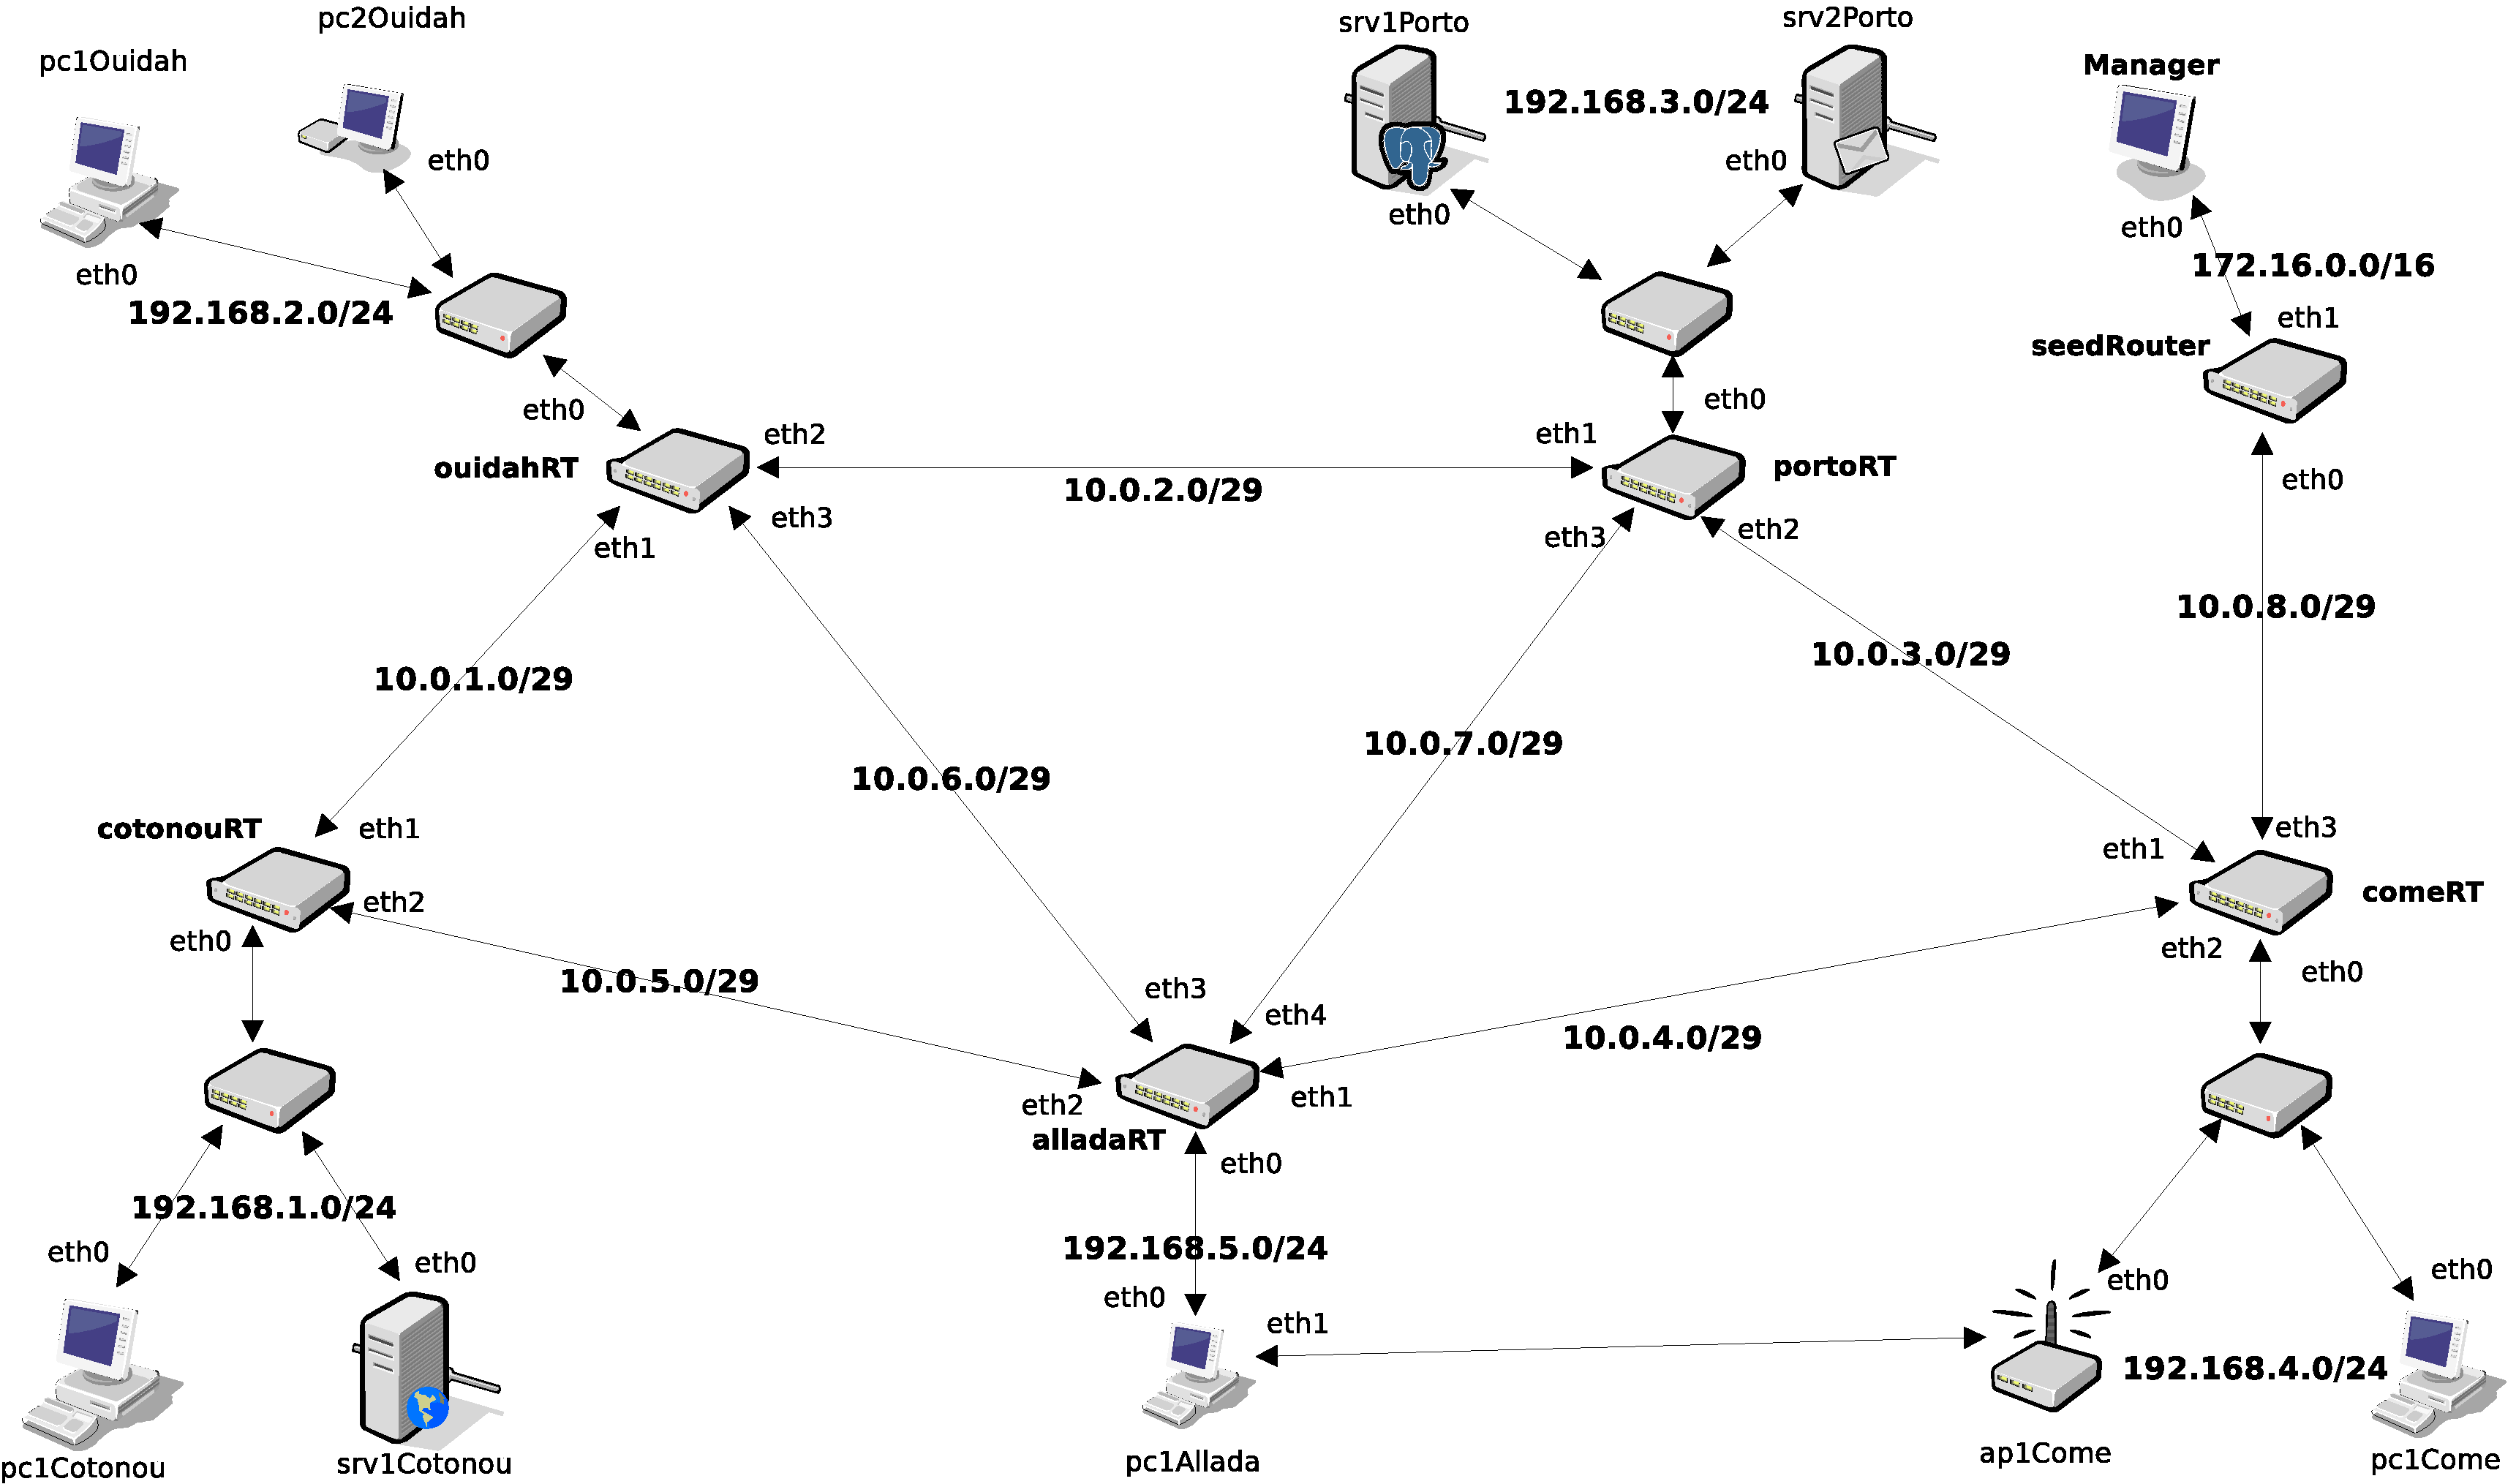
\includegraphics[scale=0.3]{images/snmp_lab.pdf}
     \caption{Modèle de réseau (crée avec NetKit) à découvrir par le seedDB} \label {fig:snmp_lab} 
        \end{center}
   \end{figure}
La figure \ref{fig:snmp_lab} (page \pageref{fig:snmp_lab}) montre le modèle de réseau crée. Ce laboratoire est constitué des équipements ayant les caractéristiques réseaux suivantes:
\begin{itemize}
\item PCs
\begin{itemize}
\item pc1Cotonou (\texttt{192.168.1.1} sur \texttt{eth0})
\item pc1Ouidah (\texttt{192.168.2.1} sur \texttt{eth0})
\item pc2Ouidah (\texttt{192.168.2.2} sur \texttt{eth0}) 
\item pc1Allada (\texttt{192.168.5.1} sur \texttt{eth0} et \texttt{192.168.4.100} sur \texttt{eth1})
\item pc1Come (\texttt{192.168.4.1} sur \texttt{eth0}) 
\end{itemize}
\item Serveurs
\begin{itemize}
\item srv1Cotonou (\texttt{192.168.1.2} sur \texttt{eth0})
\item srv1Porto (\texttt{192.168.3.1} sur \texttt{eth0}) 
\item srv2Porto (\texttt{192.168.3.2} sur \texttt{eth0})      
\end{itemize}
\item Access Point: ap1Come (\texttt{192.168.4.2} sur \texttt{eth0})
\item Routeur
\begin{itemize}
\item rtCotonou:
\begin{itemize}
\item \texttt{eth0}: \texttt{192.168.1.100}
\item \texttt{eth1}: \texttt{10.0.1.1}
\item \texttt{eth2}: \texttt{10.0.5.1}
\end{itemize}
\item rtOuidah:
\begin{itemize}
\item \texttt{eth0}: \texttt{192.168.2.100}
\item \texttt{eth1}: \texttt{10.0.1.2}
\item \texttt{eth2}: \texttt{10.0.2.2}
\item \texttt{eth3}: \texttt{10.0.6.2}
\end{itemize}
\item rtPorto:
\begin{itemize}
\item \texttt{eth0}: \texttt{192.168.3.100}
\item \texttt{eth1}: \texttt{10.0.2.3}
\item \texttt{eth2}: \texttt{10.0.3.3}
\item \texttt{eth3}: \texttt{10.0.7.3}
\end{itemize}
\item rtCome:
\begin{itemize}
\item \texttt{eth0}: \texttt{192.168.4.100}
\item \texttt{eth1}: \texttt{10.0.3.4}
\item \texttt{eth2}: \texttt{10.0.4.4}
\item \texttt{eth3}: \texttt{10.0.8.4}
\end{itemize}
\item rtAllada:
\begin{itemize}
\item \texttt{eth0}: \texttt{192.168.5.100}
\item \texttt{eth1}: \texttt{10.0.4.5}
\item \texttt{eth2}: \texttt{10.0.5.5}
\item \texttt{eth3}: \texttt{10.0.6.5}
\item \texttt{eth4}: \texttt{10.0.7.5}
\end{itemize}
\item seedRouter: 
\begin{itemize}
\item \texttt{eth0}: \texttt{10.0.8.6}
\item \texttt{eth1}: \texttt{172.16.0.6}
\end{itemize}
\end{itemize}
\end{itemize}
Le \emph{Manager} ne fait pas partie du réseau virtuel. L'adresse IP de son interface en communication avec le réseau virtuel est: \texttt{172.16.0.7}.

L'adresse \texttt{eth1} du \texttt{seedRouter} est totalement différent de celui du réseau virtuel (nous passons de la classe A à la classe B) pour éviter un conflit au niveau des adresses des interfaces \texttt{tap} et de celui du réseau virtuel de \emph{Netkit}.


Nous donnerons comme point de départ à notre algorithme, le \texttt{seedRouter}. A noter que \emph{SNMP} est déjà configuré par nos soins sur tous les équipements. Pour que depuis notre PC, nous puissions accéder au réseau virtuel à travers le \texttt{seedRouter} , il faut activer au  niveau du \texttt{seedRouter}, l'interface \texttt{tap}. 


Vu que \emph{NAV} ne supporte pas encore \emph{SNMPv3}, et que la typologie vas être découverte par \texttt{ipdevpoll} du \emph{NAV}, notre code pour plus de cohésion, implémente la classe \emph{SNMP} du \emph{NAV}, qui en fait est une extension de la classe \emph{pysnmp} (module SNMP de python).



Pour finir sur le réseau virtuel, notons que les hôtes du réseau peuvent être tout type d'équipement. Dans le cadre de cette étude nous nous sommes limités aux PCs, Switchs L2, serveurs et routeurs. Le plus important étant que l'équipement ajouté dans le réseau supporte \emph{SNMP} et soit correctement configuré.

\subsubsection{Résultats}
La classe \texttt{SeedDB} est ajouté dans le répertoire \texttt{/opt/nav-3.11.5/python/nav/seeddb}. L'appel de la classe avec les paramètres correctes donne:
\lstset{language=Python,basicstyle=\color{bookColor},basicstyle=\ttfamily,backgroundcolor=\color{White},basicstyle=\tiny} 
\begin{lstlisting}[frame=single] 
$ pwd
/opt/nav-3.11.5/python/nav/seeddb
$ sudo python seeddb.py

========================================================
=== Welcome to NAV SNMP based Network Host Discovery ===
========================================================

Enter starting router IP: 172.16.0.6
[OK] seed_router...
==============================================
==== Select SNMP version for your Network ====
==== 1 for SNMP v1                        ====
==== 2 for all versions of SNMP v2        ====
==== 3 for SNMP v3                        ====
==============================================
2
Enter community for version 2: public

Checking SNMP parameters...

[OK] SNMP parameters...
Starting device discovery

Getting all routers on the network

[OK] Routers list...

Getting all Hosts on the network

I'am affraid, looks like something went wrong with 10.0.8.6 !
===== get_local_net_address error =====
Timed out waiting for SNMP response: Manager: no response arrived before timeout


[OK] All devices list...

Setting all network Host type

[OK] Device type...

Creating bulk import file

[OK] Create bulk import file: /tmp/nav/ip_device_bulk_import_20120829013534.txt
Exiting...


\end{lstlisting} 
La classe \texttt{SeedDB} ajoute à chacun de son appel, plus de détails sur le déroulement du processus de découverte des équipements dans le fichier \texttt{/var/log/nav/autoseeddb.log} spécifié dans la classe \texttt{SeedDB}. Ce fichier journal contient beaucoup de ligne pour chaque opération: ajout dans le tableau des routeurs, regroupement des routeurs, ajout des équipements du réseau local, regroupement des équipements du réseau local, identification des types d'hôte, création du fichier d'importation. Les dernières lignes de ce fichiers peuvent donner au cas où tout c'est bien déroulé:
\lstset{language=Python,basicstyle=\color{bookColor},basicstyle=\ttfamily,backgroundcolor=\color{White},basicstyle=\tiny} 
\begin{lstlisting}[frame=single] 
$ tail -f /var/log/nav/autoseeddb.log 
[ 2012-08-29 01:35:34,900 ][ INFO     ] root - Adding line myroom:192.168.5.1:myorg:OTHER:public in file
[ 2012-08-29 01:35:34,900 ][ INFO     ] root - Adding line myroom:10.0.5.1:myorg:GW:public in file
[ 2012-08-29 01:35:34,900 ][ INFO     ] root - Adding line myroom:10.0.7.3:myorg:GW:public in file
[ 2012-08-29 01:35:34,900 ][ INFO     ] root - Adding line myroom:10.0.2.2:myorg:GW:public in file
[ 2012-08-29 01:35:34,900 ][ INFO     ] root - Adding line myroom:10.0.3.4:myorg:GW:public in file
[ 2012-08-29 01:35:34,900 ][ INFO     ] root - Closing file /tmp/nav/ip_device_bulk_import_20120829013534.txt
[ 2012-08-29 01:35:34,900 ][ INFO     ] root - Create bulk import file: /tmp/nav/ip_device_bulk_import_20120829013534.txt
[ 2012-08-29 01:35:34,900 ][ INFO     ] root - Exiting at the end of the script...
\end{lstlisting} 

Le fichier obtenu se présente comme suit:
\lstset{language=Python,basicstyle=\ttfamily,backgroundcolor=\color{fondBleu},basicstyle=\tiny} 
\begin{lstlisting}[frame=single] 
$ cat /tmp/nav/ip_device_bulk_import_20120829013534.txt
myroom:10.0.8.6:myorg:GW:public
myroom:172.16.0.7:myorg:OTHER:public
myroom:192.168.1.1:myorg:OTHER:public
myroom:192.168.1.2:myorg:OTHER:public
myroom:192.168.3.1:myorg:OTHER:public
myroom:192.168.3.2:myorg:OTHER:public
myroom:192.168.2.1:myorg:OTHER:public
myroom:192.168.2.2:myorg:OTHER:public
myroom:192.168.4.1:myorg:OTHER:public
myroom:192.168.4.2:myorg:OTHER:public
myroom:10.0.7.5:myorg:GW:public
myroom:192.168.5.1:myorg:OTHER:public
myroom:10.0.5.1:myorg:GW:public
myroom:10.0.7.3:myorg:GW:public
myroom:10.0.2.2:myorg:GW:public
myroom:10.0.3.4:myorg:GW:public
\end{lstlisting}
Les figures \ref{fig:seeddb_import_1} (page \pageref{fig:seeddb_import_1}) et \ref{fig:seeddb_import_2} (page \pageref{fig:seeddb_import_2}) montrent les résultats d'importation du fichier généré par \texttt{SeedDB} dans NAV.

\begin{figure}[H]
    \begin{center}
     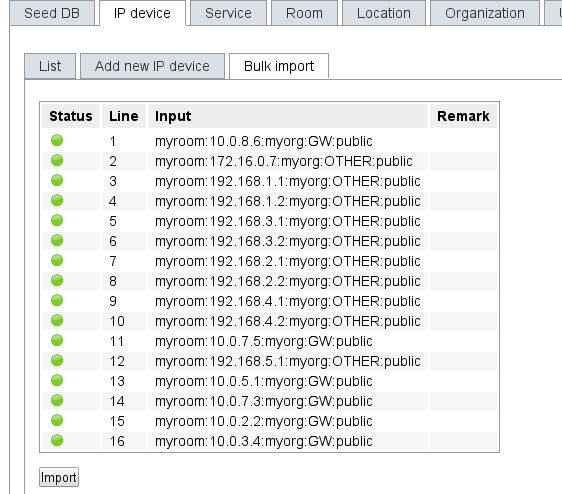
\includegraphics[scale=0.7]{images/seeddb_import.png}
     \caption{Fenêtre de confirmation de l'importation des données du fichier des équipements du réseau} \label {fig:seeddb_import_1} 
        \end{center}
   \end{figure}

\begin{figure}[H]
    \begin{center}
     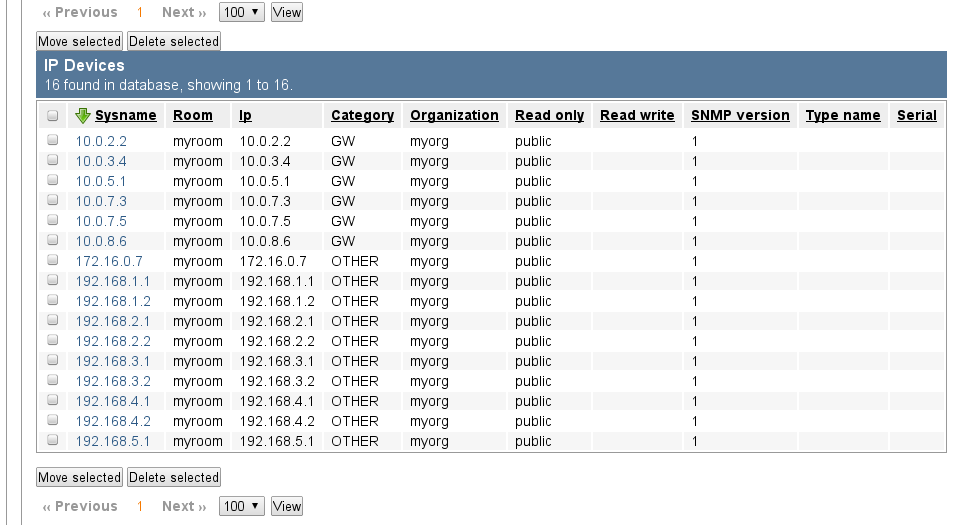
\includegraphics[scale=0.5]{images/seeddb_import_suite.png}
     \caption{Résultat de l'importation du fichier des équipements du réseau} \label {fig:seeddb_import_2} 
        \end{center}
   \end{figure}